\chapter[Sobre a proposta e a metodologia]{Sobre a proposta e a metodologia}
\label{cap-sobre-a-proposta-e-a-metodologia}

\section{Ecossistemas de startups e estudos de avaliação}
\label{section:um_breve_apanhado_sobre_ecossistemas_de_startups_e_estudos_de_avaliação}

\citeonline{Schumpeter1934} diz que empreendedores tendem a se conglomerar em uma mesmo região com o objetivo de obterem benefícios mútuos, criando clusters, que podem ser interpretados como ecossistemas, e são essenciais para o desenvolvimento local. Para \citeonline{James1953} e \citeonline{Dalcin2015} empreendedores influenciam diretamente o crescimento econômico, a oferta de empregos, a redução da pobreza e a formação e o crescimento de cidades, \citeonline{Spigel2015} afirma ainda que estudos sobre ecossistemas empreendedores se tornaram uma ferramenta importante para o estudo do empreendedorismo de alto crescimento sob o ponto de vista geográfico por esta capacidade de influenciar o desenvolvimento econômico e social de uma determinada região.

Segundo \citeonline{Dubini1989} ecossistemas são marcados pela presença de empresas, economia diversificada, boa infraestrutura de negócios e investimentos, cultura empreendedora adequada e políticas públicas que apoiem o empreendedorismo e os empreendedores. \citeonline{ranga2013triple} trás o conceito da Hélice Tripla representando ecossistemas por meio da interação entre governo, indústria e universidade.

Para \citeonline{isenberg2011introducing} um ecossistema empreendedor possui seis grandes pilares: política, finanças, cultura, suporte, capital humano e mercado, onde todos devem agir em conjunto para a criação de um ecossistema saudável e promissor, essa visão está representada na Figura \ref{figure:isenberg_ecosystem} (e adaptada para o português por \citeonline{Arruda2013}. \citeonline{schwab2015} defende que os pilares de um ecossistema são abertura de mercados, capital humano, investimento, apoio do governo, ambiente regulatório, educação, universidades e suporte cultural.

\begin{figure}[!htb]
\centering
\includegraphics[width=11cm,angle=0]{figuras/isenberg_ecosystem_ptbr}
\caption{Ecossistemas empreendedores, por \citeonline{isenberg2011introducing}}
\label{figure:isenberg_ecosystem}
\end{figure}

\citeonline{gumpert1985heart} diz que enquanto governo e academia são capazes de criar condições favoráveis para que o empreendedorismo prospere o envolvimento de indivíduos, como os empreendedores, é essencial, reforçando o modelo criado por Isenberg e indo de encontro ao modelo de Hélice Quadrupla definido por \citeonline{leydesdorff2012triple}. \citeonline{carayannis2009mode} reforça ainda a importância de considerarmos mídia e cultura como variáveis que compõem essa quarta vertente que representa a sociedade civil em um ecossistema de inovação.

Nesta linha, \citeonline{Spigel2015} define ecossistemas como a união entre elementos culturais, sociais, políticos e econômicos em uma região que, juntos, propíciam o surgimento, e o crescimento, de empresas inovadoras e encorajam novos empreendedores e demais atores a assumirem os riscos relacionados a inovação. \citeonline{Suresh2012} já concentrou seus estudos em mapear os elementos de um ecossistema que contribuem para a formação do indivíduo empreendedor, como a presença de redes que os apoiem nos momentos difíceis e sirva de exemplo para os mesmos como referências de sucesso. 

\citeonline{Motoyama2014} identificaram quatro pontos de conexões cruciais que devem acontecer para o desenvolvimento de um ecossistema: conexões entre empreendedores, conexões entre organizações de suporte, conexões entre empreendedores e organizações de suporte e conexões de suporte diversas, como eventos. Esses conceitos foram de extrema importância para este trabalho.

Reforçando a relevância das conexões em um ecossistema \citeonline{Hwang2012} fala sobre a importância dos indivíduos ``keystone'' por serem os responsáveis por quebrar barreiras sociais ``invisíveis'' que são impostas entre os diferentes atores de um ecossistema, como entre novos empreendedores e possíveis investidores ou parceiros. Os autores relatam ainda que quanto mais facilmente essas barreiras são quebradas em um determinado ecossistema mais frutífero ele será.

\citeonline{Stangler2015}, por meio da Kauffman Foundation, definem as quatro seguintes características de um ecossistema vibrante: densidade, fluídez, conectividade e diversidade. Por densidade entendem questões como a quantidade de novas empresas para cada mil habitantes, a quantidade de postos de trabalho da região e o tamanho dos setores que envolvam alta tecnologia. Para fluídez indicam questões como o fluxo populacional de uma cidade, a realocação no mercado de trabalho e a quantidade de empresas de alto crescimento. Para conectividade os indicadores podem ser relacionados a redes de investidores, conectividade entre programas e a quantidade de spin-offs, como são chamadas as empresas que foram criadas por pessoas relacionadas a outras empresas mais antigas e estabelecidas, geralmente criadas por ex-funcionários. Por fim, diversidade idealmente pode ser entendida como a quantidade de especializações econômicas na região, a taxa de mobilidade social e dados relativos a imigração. O artigo em si não descreve um arcabouço para avaliação de ecossistemas, mas define bons indicadores que podem ser utilizados por outros trabalhos.

\citeonline{Feld2012} desenvolveu a ``Teoria de Boulder'' a qual ele define quatro regras para um ecossistema de qualidade: 1) Precisa ser liderado por empreendedores; 2) Os líderes precisam assumir um compromisso a longo prazo para com o ecossistema; 3) O ecossistema precisa ser inclusivo para qualquer pessoa que queira participar; e 4) O ecossistema precisa ter atividades contínuas que engajem a comunidade empreendedora local. Ele também elencou alguns atores que compõem e são de grande importância para ecossistemas como empreendedores, governo, universidades, investidores, mentores, provedores de serviços e grandes empresas já estabelecidas localmente. Outro fator interessante é que o autor enxerga ecossistemas empreendedores como organismos vivos em constante evolução, e não estruturas bem definidas e estáticas. Com base nesse princípio ele também faz a divisão de atores entre ``semeadores'' (seeders, aqueles que fomentam e contribuem para o crescimento do ecossistema) e ``consumidores'' (feeders, todos aqueles que não atuam como semeadores e se beneficiam com o crescimento do ecossistema).  

Partindo para a avaliação de ecossistemas os pesquisadores \citeonline{Arnaud2009} e \citeonline{Ahmad2007} apresentaram metodologias centradas em três grandes pilares: 1) Fatores determinantes, envolvendo indicadores de ambiente regulatório, acesso a capital, cultura e capacidades empreendedoras; 2) Performance, englobando indicadores relativos ao desenvolvimento das empresas da região; e 3) Impacto, envolvendo indicadores sociais como índices de geração de empregos, crescimento econômico e redução da pobreza.

Com base nos pilares definidos por \citeonline{Arnaud2009} o pesquisador brasileiro \citeonline{Arruda2013} desenvolveu um estudo sobre o ecossistema de startups brasileiro, como resultados obtiveram visões sobre o modelo regulatório brasileiro, as nossas condições de mercado, o acesso a financiamento, a criação e a difusão de conhecimento, a capacidade e a cultura empreendedora e demais peculiaridades regionais do Brasil. O trabalho também lista em anexo todas as variáveis mapeadas para o trabalho e suas fontes, que foram de grande importância para este trabalho. Nas recomendações de trabalho futuro mencionam a dificuldade em conversar sobre experiências de fracasso com os empreendedores brasileiros, em especial com aqueles que ainda não obtiveram algum caso de sucesso, talvez esse problema se repita no contexto do Distrito Federal e pode ser interpretado como reflexo de imaturidade no ecossistema. A metodologia utilizada por Arruda se assemelha a deste trabalho por se tratar de uma abordagem mista (quantitativa e qualitativa) e ter como base entrevistas com atores relevantes para o ecossistema.

\citeonline{Hermann2015}, por meio do ``The Global Startup Ecosystem Ranking'' e da ``Compass'', realizaram um estudo sobre ecossistemas com base em seis pilares principais: performance, financiamento, alcance de mercado, talento, experiência em startups e índice de crescimento. 

\citeonline{Kutt2013}, por meio de uma análise quantitativa de diversas bases de dados locais e globais fez uma comparação do ecossistema de startups da Estônia em um contexto internacional, comparando-o como Finlândia, Taiwan, Israel, Coreia e Singapura. O autor também fez um estudo por meio da análise de dados de redes sociais para obter uma visualização das estruturas sociais do ecossistema da Estônia e identificar como os atores se conectam entre si. Essa metodologia também se aproxima da forma como este trabalho fora abordado.

A \citeonline{indiceglobaldoempreendedorismo} publica anualmente o Índice de Cidades Empreendedoras e tem sua análise de ecossistemas baseada em sete pilares: ambiente regulatório, infraestrutura, mercado, acesso a capital, inovação, capital humano e cultura empreendedora. De acordo com os índices de 2015 e 2016 Brasília demonstrou uma melhora significativa em alguns dos pilares mas, também, piora em outras, como demonstrado pela Figura \ref{figure:ici20152016}. 

\begin{figure}[!htb]
	\centering
	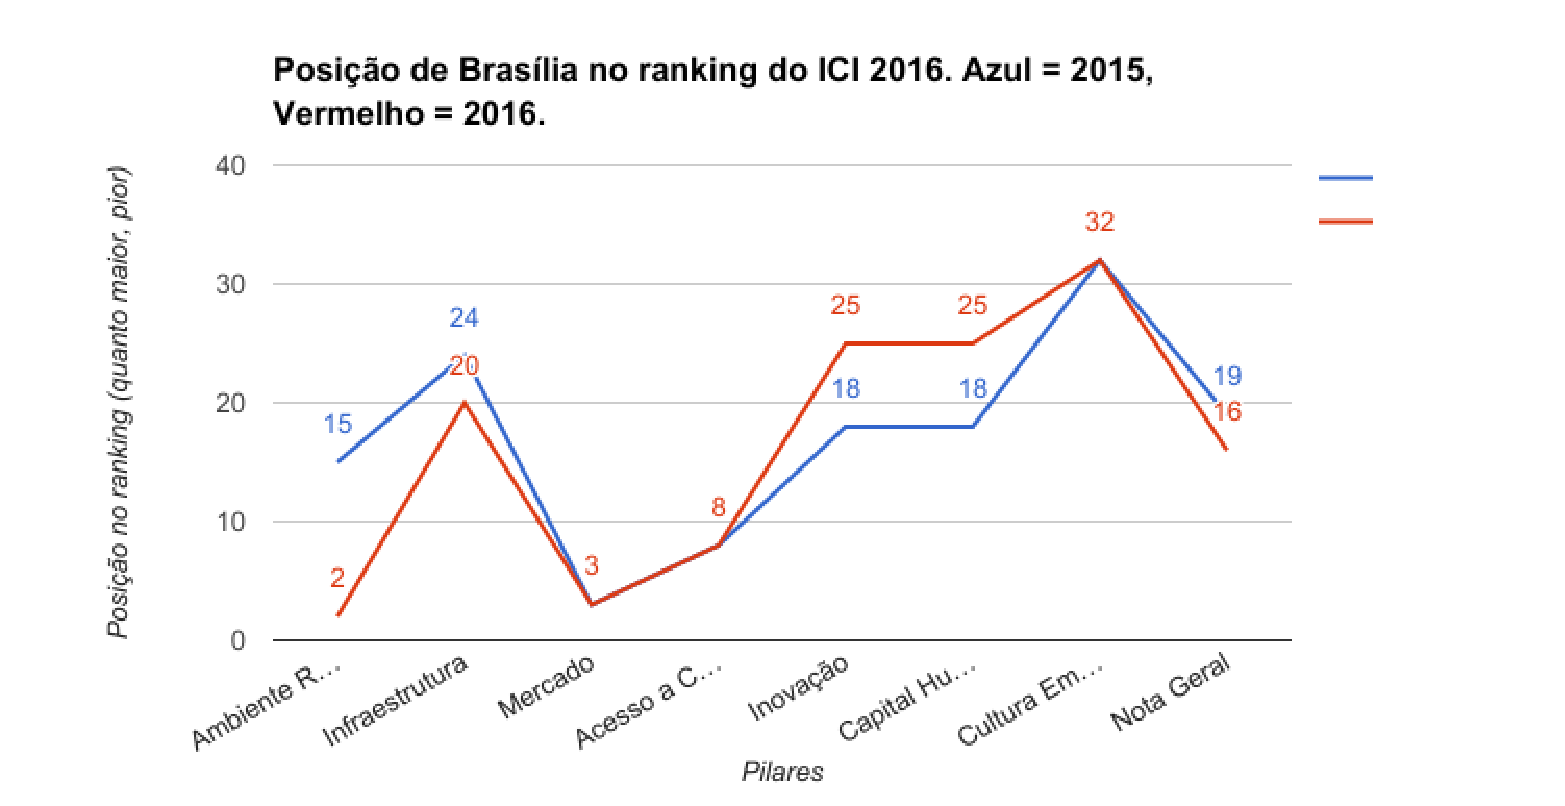
\includegraphics[width=11cm,angle=0]{figuras/ici20152016}
	\caption{Indicadores de Brasília no Índice de Cidades Empreendedoras}
	\label{figure:ici20152016}
\end{figure}

\section{A metodologia}
\label{section:a_metodologia}

Muitos dos estudos anteriores tiveram como bases a análise de dados quantitativa, embora outros pesquisadores optem por abordagens qualitativas ou mistas. \citeonline{Maxwell2013} define pesquisas qualitativas como pesquisas que tem como objetivo ajudar o pesquisador a entender as perspectivas dos indivíduos estudados - o mundo pelo ponto de vista de quem faz parte do objeto de estudo e não do ponto de vista do pesquisador. É uma forma de entender como essas perspectivas moldam e influenciam o contexto estudado e como diversos fatores se envolvem com os fenômenos e relacionamentos em estudo. 

Seguindo essa linha, \citeonline{Merriam1991} defende que o processo e o conhecimento obtidos durante o estudo são mais importantes do que os resultados finais, isso é possível graças a uma abordagem flexível que tem como base uma abordagem visual, falada ou textual, ao invés de análises puramente estatísticas e numéricas, como é o caso dos estudos quantitativos. Maxwell diz ainda que o pesquisador que opta por trabalhar com a abordagem qualitativa busca enxergar o mundo através de pessoas, situações, eventos e processos que os conectam. Alguns dos pontos fortes de uma Pesquisa Qualitativa de acordo com Maxwell estão representados pela Tabela \ref{table:objetivos_intelectuais_segundo_maxwell} e alguns dos objetivos pela Tabela \ref{table:pontos_fortes_segundo_maxwell}.

\begin{table}[!htb]
	\centering
	\begin{tabular}{ | p{3cm} | p{12cm} | }
		\hline
		1 & Entender o significado, de acordo com os participantes do estudo, dos eventos, situações, experiências e ações em que eles se envolvem ou engajam. \\ \hline
		2 & Entender os contextos particulares em que os participantes do estudo atuam e como esses contextos impactam em suas decisões. \\ \hline
		3 & Entender o processo o qual eventos e ações acontecem. \\ \hline
		4 & Identificar fenômenos e influências não previstos gerando novas teorias fundamentadas em dados sobre o objeto estudado. \\ \hline
	\end{tabular}
	\caption{Pontos fortes de uma Pesquisa Qualitativa}
	\label{table:objetivos_intelectuais_segundo_maxwell}
\end{table}

\begin{table}[!htb]
	\centering
	\begin{tabular}{ | p{3cm} | p{12cm} | }
		\hline
		1 & Gerar teorias e resultados que sejam válidos e compreensíveis tanto para as pessoas que estão sendo estudadas como também para outras pessoas, que possam ou não ser pesquisadores. \\ \hline
		2 & Melhorar práticas, programas ou políticas existentes ao invés de simplesmente avalia-las, por esse motivo é importante entender os processos e contextos específicos dessas ações e como elas são vistas pelos participantes da pesquisa. \\ \hline
		3 & Engajar-se em ações participativas, colaborativas ou com foco na comunidade junto com os participates do estudo. \\ \hline
	\end{tabular}
	\caption{Alguns dos objetivos de uma Pesquisa Qualitativa}
	\label{table:pontos_fortes_segundo_maxwell}
\end{table}

\citeonline{Kon2014}, criador da metodologia utilizada como base deste trabalho, explora ambas as abordagens qualitativa e quantitativa com o objetivo de mensurar a maturidade de um determinado ecossistema de startups utilizando como base entrevistas com atores dos ecossistemas locais, seguindo técnicas de estudos qualitativos, juntamente com a exploração de dados estatísticos acerca do ecossistema. Assim como \citeonline{Frenkel2014}, Kon também se propôs a criar uma arcabouço conceitual do ecossistema em estudo e aplicou a referida metodologia nas cidades de Tel Aviv (Israel), Nova Iorque (EUA) e São Paulo, outros pesquisadores a aplicaram em Belém e outro estudante de graduação a está aplicando em Belo Horizonte. 

A forma como a metodologia fora construída permite que os pesquisadores realizem comparações diretas entre ecossistemas ao diferencia-los por níveis (nascente, crescente, maduro e auto-sustentável). Os resultados das aferições realizadas em Tel Aviv estão disponíveis na Figura \ref{figure:mapa_conceitual_tel_aviv} e em São Paulo na Figura \ref{figure:mapa_conceitual_sao_paulo}.

A maior vantagem da metodologia proposta se dá por oferecer uma forma de obter conhecimento a partir das visões daqueles que melhor o entendem e lidam com o ecossistema de startups local - os próprios empreendedores. Ao dar uma maior prioridade a esse tipo de abordagem ao invés de uma análise puramente quantitativa torna-se possível obter uma visualização mais realista e próxima de quais são as características do ecossistema em estudo como um todo, além de contornar a falta de bases de dados alimentadas de forma sistemática de ecossistemas menos estruturadas e maduros. Essa abordagem também aumenta as chances de que a atividade de pesquisa entregará valor ao pesquisador mesmo quando alguns dos fatores propostos pela metodologia não são aplicáveis no ecossistema em análise.

Dentre as técnicas de pesquisa qualitativa que serão utilizadas está a Teoria Fundamentada em Dados, segundo \citeonline{Glaser1999} a mesma se trata de uma série de conhecimentos que são desenvolvidos de forma indutiva durante o estudo e com uma forte integração com os dados coletados, ela quem torna possível que as perguntas que motivam este estudo sejam respondidas com base nas entrevistas realizadas com empreendedores e atores do ecossistema de startups do Distrito Federal.

\subsection{Os níveis de maturidade de um Ecossistema}
\label{subsection:niveis_de_maturidade_de_um_ecossistema}

Além de elaborar o mapa do ecossistema a Metodologia tem como um dos seus objetivos classificar Ecossistemas entre quatro diferentes níveis de maturidade. Os níveis são os seguintes:

\begin{description}
  \item [Nascente (M1):] quando há um Ecossistema com algumas Startups presentes no mercado, alguns investimentos concretizados e algumas iniciativas com o objetivo de estimular ou fomentar o Ecossistema sendo realizadas mas não há reconhecimento ou as Startups não possuem representatividade nos índices de geração de emprego e renda da região.

  \item [Crescente (M2):] quando há algumas Startups estabelecidas como empresas sólidas e o Ecossistema como um todo possui representatividade notável na economia regional e nos índices de empregos. Para se enquadrar como Crescente todos fatores essenciais e cerca de 30\% dos fatores derivados deverão ser classificadas como nível L2.

  \item [Maduro (M3):] quando existem algumas centenas de Startups em atividade, sendo algumas reconhecidas internacionalmente e com negócios realizados globalmente, um histórico relevante de investimentos concretizados dentro do Ecossistema e pelo menos uma geração de empreendedores bem sucedidos que se tornaram líderes, mentores, referências e investidores-anjo para os novos empreendedores, ajudando-os a crescer. Além dessas características, para ser considerado como um Ecossistema Maduro, todos os fatores essenciais e pelo menos 50\% dos fatores derivados devem ser classificadas como nível L2 e, no mínimo, 30\% de todos os fatores devem estar enquadrados no nível L3.

  \item [Sustentável (M4):] quando o número de Startups em atividade e de aquisições e/ou investimentos dentro do Ecossistema ultrapassam a casa dos milhares, há no mínimo duas gerações de empreendedores bem sucedidos que iniciaram suas carreiras com Startups de tecnologia presentes, uma rede de empreendedores comprometidos com o desenvolvimento do Ecossistema à longo prazo, um ambiente inclusivo com muitos eventos envolvendo temáticas que fomentem a cultura empreendedora e o mercado local e a presença de uma alta quantidade de profissionais de alta qualidade técnica. Para possuir esse estágio de maturidade, todos os fatores essenciais devem ser classificados como nível L3 e pelos menos 80\% dos fatores derivados também como nível L3.
\end{description}

\subsection{Fatores que formam um Ecossistema}
\label{subsection:fatores_que_formam_um_ecossistema}

Após vasta pesquisa bibliográfica e entrevistas com mais de 50 pessoas chaves para os Ecossistemas de Tel-Aviv e São Paulo foram definidos cerca de 21 fatores que os compõem e fazem parte do Arcabouço Teórico de um Ecossistema, descrito na subseção \ref{subsection:arcabouco_conceitual_e_modelo}. Com o objetivo de classifica-los com o fim de facilitar possíveis comparações e o cálculo final da maturidade do Ecossistema foram definidas as seguintes métricas e níveis para cada um dos fatores representados na Tabela \ref{table:metricas_de_classificacao_dos_fatores}, vale ressaltar que os fatores que contém o símbolo \"*\" antes de seu nome são os fatores essenciais, os restantes são considerados fatores derivados. Uma descrição de cada um dos fatores citados está disponível no Apêndice \ref{apendices:fatores_de_um_ecossistema}.

\begin{table}
\centering
\begin{tabular}{ | c | c | c | c |}
\hline
\thead{Fator} & \thead{L1} & \thead{L2} & \thead{L3} \\
\hline
Estratégias de Saída*                                      &     00     &     01     &    >=2      \\
\hline
Mercado Global*                                            &    <10\%   &   10-40\%  &    >40\%    \\
\hline
Empreendedorismo nas Universidades*                        &    <02\%   &   02-10\%  &    >10\%    \\
\hline
Qualidade de Mentores                                      &    <10\%   &   10-50\%  &    >50\%    \\
\hline
Burocracia                                                 &    >40\%   &   10-40\%  &    <10\%    \\
\hline
Gastos com impostos                                        &    >50\%   &   30-50\%  &    <30\%    \\
\hline
Qualidade das Aceleradoras                                 &    <10\%   &   10-50\%  &    >50\%    \\
\hline
Acesso à investimento em US\$ por ano                      &    <200M   &   200M-1B  &    >1B      \\
\hline
Qualidade do Capital Humano                                &    >20th   &   15-20th  &    <15th    \\
\hline
Valores Culturais para o Empreendedorismo*                 &    <0.5    &   0.5-0.75 &    >0.75    \\
\hline
Processos de Transferência de Tecnologia                   &    <4.0    &   4.0-5.0  &    >5.0     \\
\hline
Conhecimento das Metodologias                              &    20\%    &   20-60\%  &    >60\%    \\
\hline
Atores da Mídia com foco no Empreendedorismo               &    <03     &   03-05    &    > 05     \\
\hline
Eventos relacionados à Startups*                           &   mensal  &   semanal   &    diário    \\
\hline
Dados do Ecossistema e Pesquisas*                          &    nada    & parciais    & disponíveis \\
\hline
Gerações do Ecossistema*                                   &     00     &    0.1     &    02       \\
\hline
Número de Startups*                                        &    <200    &   200-1k   &    >1k      \\
\hline
\makecell{Acesso à investimento em quantidade \\de negócios/ano}&\makecell{<50}&\makecell{50-300}&\makecell{>300}\\
\hline
Acesso à investimento anjo em quantidade/ano*              &    <05     &   05-50    &    >50      \\
\hline
Incubadoras e Parques Tecnológicos                         &     01     &    02-05   &    >5       \\
\hline
Presença de Empresas de Alta Tecnologia*                   &    <02     &   02-10    &    >10      \\
\hline
Influência de Empresas já estabelecidas                    &    <02     &   02-10    &    >10      \\
\hline
\end{tabular}

\caption{Métricas de classificação dos Fatores que compõem um Ecossistema}
\label{table:metricas_de_classificacao_dos_fatores}
\end{table}

Também fora desenvolvida uma versão mais enxuta do modelo de avaliação proposto, com foco em apenas oito fatores ao invés de 21. Os parâmetros utilizados estão representados na Tabela \ref{table:metricas_de_classificacao_versao_enxuta} e a importância de cada um dos fatores na Tabela \ref{table:valor_das_metricas_de_classificacao_versao_enxuta}. Vale ressaltar que na versão enxuta o grupo InovaSampa optou por definir os valores esperados para cada indicador de acordo com o nível de maturidade do ecossistema, ao invés de classifica-los individualmente em quatro diferentes níveis para, então, ponderar todos os indicadores em conjunto para se obter a maturidade do ecossistema.

\begin{table}
\centering
\begin{tabular}{ | c | c | c | c | c |}
\hline
\thead{Fator} & \thead{Nascente} & \thead{Crescente} &\thead{Maduro}& \thead{Sustentável} \\
\hline
\makecell{Estratégias\\de saída}&nenhum&poucos&\makecell{várias aquisições\\e fusões mas\\poucos IPO's}&\makecell{várias aquisições\\e fusões e\\muitos IPO's}\\
\hline
\makecell{Empreendedorismo\\nas universidades}&\makecell{<02\%}&\makecell{02-10\%}&\makecell{10\%}&\makecell{>10\%} \\
\hline
\makecell{Investimento Anjo}&irrelevante &   irrelevante  &  alguns & muitos    \\
\hline
\makecell{Valores culturais\\para o\\empreendedorismo}&<0.5    &   0.5-0.6 &    0.6-0.7 & > 0.7    \\
\hline
\makecell{Atores da mídia\\com foco no\\empreendedorismo}&nenhum     &   alguns    &    muitos & todos     \\
\hline
\makecell{Dados do ecossistema\\e pesquisas}&nenhum    & nenhum & parciais    & completos \\
\hline 
\makecell{Gerações do\\ecossistema}&0& 0     &    1-2     &    >= 3       \\
\hline
\makecell{Eventos}&mensais & semanais & diários  & > diários \\
\hline
\end{tabular}

\caption{Indicadores da versão enxuta}
\label{table:metricas_de_classificacao_versao_enxuta}
\end{table}

\begin{table}
\centering
\begin{tabular}{ | c | c | c | c | c |}
\hline
\thead{Fator} & \thead{Nascente} & \thead{Crescente} &\thead{Maduro}& \thead{Sustentável} \\
\hline
\makecell{Estratégias\\de saída}&\cellcolor[rgb]{0.91,0.84,0.42}&\cellcolor[rgb]{0.91,0.84,0.42}&\cellcolor[rgb]{0.13,0.67,0.8}&\cellcolor[rgb]{0.13,0.67,0.8} \\
\hline
\makecell{Empreendedorismo\\nas universidades}&\cellcolor[rgb]{0.13,0.67,0.8}&\cellcolor[rgb]{0.13,0.67,0.8}&\cellcolor[rgb]{0.55,0.71,0.0}&\cellcolor[rgb]{0.91,0.84,0.42} \\
\hline
\makecell{Investimento Anjo}&\cellcolor[rgb]{0.91,0.84,0.42}&\cellcolor[rgb]{0.91,0.84,0.42}&\cellcolor[rgb]{0.55,0.71,0.0}&\cellcolor[rgb]{0.13,0.67,0.8} \\
\hline
\makecell{Valores culturais\\para o\\empreendedorismo}&\cellcolor[rgb]{0.13,0.67,0.8}&\cellcolor[rgb]{0.13,0.67,0.8}&\cellcolor[rgb]{0.13,0.67,0.8}&\cellcolor[rgb]{0.55,0.71,0.0} \\
\hline
\makecell{Atores da mídia\\com foco no\\empreendedorismo}&\cellcolor[rgb]{0.91,0.84,0.42}&\cellcolor[rgb]{0.55,0.71,0.0}&\cellcolor[rgb]{0.13,0.67,0.8}&\cellcolor[rgb]{0.13,0.67,0.8} \\
\hline
\makecell{Dados do ecossistema\\e pesquisas}&\cellcolor[rgb]{0.91,0.84,0.42}&\cellcolor[rgb]{0.91,0.84,0.42}&\cellcolor[rgb]{0.55,0.71,0.0}&\cellcolor[rgb]{0.13,0.67,0.8} \\
\hline 
\makecell{Gerações do\\ecossistema}&\cellcolor[rgb]{0.91,0.84,0.42}&\cellcolor[rgb]{0.91,0.84,0.42}&\cellcolor[rgb]{0.55,0.71,0.0}&\cellcolor[rgb]{0.13,0.67,0.8} \\
\hline
\makecell{Eventos}&\cellcolor[rgb]{0.13,0.67,0.8}&\cellcolor[rgb]{0.13,0.67,0.8}&\cellcolor[rgb]{0.55,0.71,0.0}&\cellcolor[rgb]{0.91,0.84,0.42} \\
\hline \hline
\makecell{Legenda}&\cellcolor[rgb]{0.91,0.84,0.42}Não importante&\cellcolor[rgb]{0.55,0.71,0.0}Importante&\cellcolor[rgb]{0.13,0.67,0.8}Muito importante&\cellcolor[rgb]{1,1,1}  \\
\hline
\end{tabular}

\caption{Importância das métricas da versão enxuta}
\label{table:valor_das_metricas_de_classificacao_versao_enxuta}
\end{table}

\subsection{Adaptações para o trabalho}
\label{subsection:adaptacoes_para_o_trabalho}

Ambas as versões completa, com os 21 fatores, e a enxuta, com 8, não se mostram adequadas para o contexto do ecossistema de startups do Distrito Federal pela falta de dados confiáveis que possam ser utilizados portanto este trabalho estará concentrado em uma análise qualitativa sobre o ecossistema e apenas os fatores quantitativos a seguir serão considerados:

 \begin{table}
\centering
\begin{tabular}{ | c | c | c | c | c |}
\hline
\thead{Fator} & \thead{Nascente} & \thead{Crescente} &\thead{Maduro}& \thead{Sustentável} \\
\hline
\makecell{Estratégias\\de saída}&nenhum&poucos&\makecell{várias aquisições\\e fusões mas\\poucos IPO's}&\makecell{várias aquisições\\e fusões e\\muitos IPO's}\\
\hline
\makecell{Investimento Anjo}&\makecell{irrelevante}&\makecell{irrelevante}  &\makecell{alguns} & \makecell{muitos}    \\
\hline
\makecell{Cultura\\Empreendedora}&\makecell{0-4}&\makecell{4-6}&\makecell{6-8}&\makecell{8-10}\\
\hline
\makecell{Atores da mídia\\com foco no\\empreendedorismo}&\makecell{nenhum}     &   \makecell{alguns}    &    \makecell{muitos} & \makecell{todos}     \\
\hline
\makecell{Dados do ecossistema\\e pesquisas}&\makecell{nenhum}    & \makecell{nenhum} & \makecell{parciais}    & \makecell{completos} \\
\hline 
\makecell{Gerações do\\ecossistema}&\makecell{0}& \makecell{0}     &    \makecell{1-2}     &    \makecell{>= 3}       \\
\hline
\makecell{Eventos}&\makecell{mensais} & \makecell{semanais} & \makecell{diários}  & \makecell{> diários} \\
\hline
\makecell{Incubadoras \\e\\Parques Tecnológicos}    & \makecell{0} &    \makecell{01}     &    \makecell{02-05}   &    \makecell{>5}    \\
\hline
\makecell{Ambiente regulatório}&\makecell{0-3}&\makecell{3-5}&\makecell{5-8}&\makecell{8-10}\\
\hline
\end{tabular}

\caption{Indicadores utilizados na pesquisa}
\label{table:metricas_de_classificacao_utilizadas}
\end{table}

O fator \"Valores culturais para o empreendedorismo\" fora substituído por \"Cultura Empreendedora\" e ao invés de utilizar um dado proveninente do Global Entrepreneurship Index, referente ao Brasil e não aos ecossistemsa locais, fora utilizado o indicador de mesmo do Índice de Cidades Empreendedoras, construído pela Endeavor. O fator \"Incubadoras e Parques Tecnológicos\" foi inserido por se tratar de um dado conhecido. 

\subsection{O arcabouço conceitual e o Mapa de um Ecossistema}
\label{subsection:arcabouco_conceitual_e_modelo}

Com base nos mesmos fatores descritos na subseção anterior, na relevância de cada um dos fatores descritos, de acordo com a visão das pessoas que compõem o próprio ecossistema e nas informações disponibilizadas por outros pesquisadores ou bases de dados foi elaborado um arcabouço conceitual de um ecossistema, representado pela Figura \ref{figure:arcabouco_teorico_de_um_ecossistema}. Nas Figuras \ref{figure:mapa_conceitual_tel_aviv}, \ref{figure:mapa_conceitual_sao_paulo} o Mapa do Ecossistema de São Paulo, ambos tendo como base o mesmo arcabouço conceitual. Os três Mapas Conceituais estão disponíveis no Anexo \ref{anexo:mapas_concentuais_do_inovasampa}.

\section{Aplicação da Metodologia e Protocolo}
\label{section:aplicacao_da_metodologia}

A aplicação da Metodologia foi dividida em três etapas:

\begin{enumerate}
  \item Entrevistas e Observações
  \item Codificação dos Dados
  \item Análises e Conclusões
\end{enumerate}

A primeira, de entrevistas e observações, se deu por meio da observação de diversos eventos e espaços com empreendedores que compõem o ecossistema de startups do Distrito Federal e das pessoas que o constroem e por meio de entrevistas individuais com pessoas atuantes no Ecossistema com objetivo de entender seu contexto pessoal e profissional, bem como suas visões sobre a realidade e as dinâmicas do ecossistema como um todo, quais os seus pontos fortes e fracos, seus maiores problemas, como diversas instituições e pessoas interagem entre si afim de fomenta-lo e quais ações poderiam ser tomadas afim de melhorá-lo.

Com a codificação dos dados todas as informações levantadas pela primeira etapa foram catalogadas em tabelas com o objetivo de se tornarem referências para as etapas de análises e conclusões e futuras pesquisas bem como documentar todo o processo que foi realizado. 

Com as análises dos dados e sua adequação nos fatores pré-definidos será possível mensurar a maturidade do ecossistema com o objetivo de gerar as conclusões da pesquisa, que se concentrarão em explicitar o atual estágio do Ecossistema de acordo com a Metodologia utilizada, em realizar comparações com outros ecossistemas e identificar uma série de ações que podem ser tomadas para aprimorar determinados pontos.

\subsection{Questões de Pesquisa}
\label{subsection:questoes_de_pesquisa}

\begin{itemize}
  \item Questão de Pesquisa 1: Quais são as características socioculturais de Brasília que promovem ou inibem o empreendedorismo?
  \item Questão de Pesquisa 2: Quais são os mecânismos institucionais de Brasília que promovem ou dificultam o Empreendedorismo?
  \item Questão de Pesquisa 3: Quais são os mecânismos educacionais de Brasília que promovem o Empreendedorismo?
  \item Questão de Pesquisa 4: Como os fatores tecnológicos influenciam o sucesso ou fracasso das Startups de Brasília? Qual o papel executado pela comunidade e pelo Software Livre?
  \item Questão de Pesquisa 5: Qual a relação do empreendedor de Brasília com as opções de investimento disponíveis e como elas influenciam o Ecossistema?
  \item Questão de Pesquisa 6: Quais ações devem ser tomadas no Ecossistema de Brasília para que ele cresça?
\end{itemize}

Vale ressaltar que muitas delas são exatamente como as definidas no mapeamento de Tel-Aviv realizado por \citeonline{Kon2014} e de São Paulo por \citeonline{MonnaSantos2015}.

\subsection{Escolha dos Entrevistados}
\label{subsection:escolha_dos_entrevistados}

É de extrema importância que os entrevistados sejam atuantes e bem conectados com o ecossistema de startups do Distrito Federal como um todo e, em sua maior parte, Empreendedores mas Professores, Servidores e Agentes Públicos, Investidores, Representantes de Incubadoras e Aceleradoras e Estudantes também serão consultados. A meta é que sejam entrevistados cerca de 20 pessoas destes grupos.

Assim como sugerido pelos criadores da metodologia, para a escolha dos entrevistados fora aplicada a metodologia bola de neve. Primeiramente, foram definidos algumas pessoas com alto histórico de contribuição e participação no ecossistema e que faziam parte da rede de contatos das pessoas envolvidas com a pesquisa e foram solicitadas recomendações de quais pessoas deveriam fazer parte desta pesquisa e, se possível, solicitado uma introdução entre essas pessoas. Ao fim de cada entrevista esse processo também foi repetido.

\subsection{Condução das Entrevistas}
\label{subsection:conducao_das_entrevistas}

Foi dada liberdade ao entrevistado de escolher o local da entrevista, em sua maior parte elas aconteceram no próprio local de trabalho da pessoa mas também foram utilizadas cafeterias e softwares de videoconferência como Skype e Google Hangout. Todas foram devidamente gravadas em aúdio com nuência do empreendedor.

Foi tomado cuidado para que as entrevistas não fossem muito longas, a maior parte não extrapolando o prazo de 40 minutos a 1 hora de duração. Para guiar o entrevistador foram estabelecidas uma série de perguntas que foram realizadas aos entrevistados com o objetivo de obter respostas que respondam às questões de pesquisa estabelecidas em \ref{subsection:questoes_de_pesquisa}.

Não necessariamente as entrevistas seguiram de forma rígida todas as perguntas definidas no roteiro, de acordo com o perfil do entrevistado ou a evolução das conversas elas foram adaptadas. Como a entrevista fora conduzida ou a linguagem utilizada não são de grande importância, desde que a maior parte das questões fossem respondidas, mesmo que de forma indireta. Em muitos casos o próprio entrevistado respondeu algumas delas durante outras perguntas. 

Todas as perguntas e o roteiro sugerido estão disponíveis no Apêndice \ref{apendices:perguntas_das_entrevistas}. Os convites foram via email, LinkedIn, redes sociais, telefone ou pessoalmente.

\subsection{Transcrição, Codificação e Interpretação dos Dados}
\label{subsection:codificacao_e_interpretacao_dos_dados}

Após a realização de cada Entrevista a transcrição e codificação das entrevistas fora feita utilizando o software MAXQDA\footciteref{MaxQDA}, a escolha por esse software se deu após análise das opções disponíveis, pelo suporte oferecido pela empresa criadora da solução e por recomendação de um dos criadores da metodologia.